\subsection{Train Models for Audible Events} 
\label{sec:audiotrain}

Once we download audio samples for each of the event terms in the vocabulary,
we can train audio models for each event. 

\subsubsection{Feature selection}
To train audio models, first we need to find a good way (features) 
to describe the audio data. 
%Many features have been proposed by researchers in the past. 
We view an audio clip as a sequence of logically overlapping frames, 
each comprised of fix number of sample points, as in \fig{fra}.
The amount of overlap is a parameter of the model.
A frame is the basic unit of feature extraction, 
in either time or frequency domain. 

\begin{figure}[th]
\centering
\epsfig{file=figures/frame.eps,width=0.8\columnwidth}
\caption{Overlapping Audio Frames}
\label{fig:fra}
\end{figure}

%Existing works \cite{1561288,1621215,mitrovic2010features,4761905} reported
%that, in the frequency domain, the mel-frequency cepstrum coefficients (MFCC) 
%feature is a widely-used feature which is a cepstral representation 
%of the audio clip, i.e., a non-linear spectrum-of-a-spectrum. 
%It is fairly robust because it closely resembles the human auditory system's
%response to different frequency bands.
%
%In the time domain, short-time energy is the energy measure of a short segment
%of sound. It has been shown to be a simple and 
%effective feature to distinguish active voice against silence in
%speech processing \cite{1181092}. 
%
%Zero crossing rate (ZCR) is a temporal feature which measures the rate 
%at which the signal transits from positive to negative or back. 
%ZCR can be used to distinguish meaningful events from environmental noise, 
%since environmental noise usually has a larger ZCR.
%
%In our work, we use short time energy to remove ambient noises first. 
%Then, we combine ZCR and MFCC as features, which will be used in the
%audible events modeling next.
%
%\subsubsection{Model selection}
%GMM and HMM are mostly used in these kind of problems. We will discuss both of them in the following sections.

\subsubsection{Event models}
In this paper, every audible event in the vocabulary is modeled as one or
more GMMs. A GMM is a weighted sum of $M$ Gaussian density function, 
which is given by:
\begin{equation}
P(\mathbf{x}|\mathbf{\Theta}) = \sum_{i = 0}^{M - 1} c_i\prod_{d=0}^{D-1} \frac{1}{\sqrt{(2\pi)}\sigma_{i,d}}e^{-\frac{1}{2\sigma_{i,d}^{2}}(x_d-\mu_{i,d})^2},
\label{eqn:gmm}
\end{equation}
where $\mathbf{x}$ is a $D$-dimensional variable representing
the feature vector, $\Theta$ is the parameters of GMM, 
including $\mathbf{c}$, $\mathbf{\mu}$ and $\mathbf{\sigma}$.
$c_i$ is the weight of the $i^{th}$ mixture, with the following constraint:
\begin{equation}
\sum_{i=0}^{M-1}c_i=1,
\end{equation}
while $\mu_{i,d}$ and $\sigma_{i,d}$ are the mean and standard deviation 
of the dimension $d$ of the $i^{th}$ mixture.

\subsubsection{Model training}
The audio samples downloaded for each event term in the vocabulary, 
such as ``dog'' may sound very different, either because there are various
aspects of an event, or in the case of ``dog'', simply because there are
different species -- {\em bull dogs} certainly sound very 
different from {\em chihuahuas}.
To accurately models each event, in this paper, we aim to derive multiple
GMMs, each for a separate aspect of an event. 

Before we do the actual training, we first remove ambient noise from
the training clips. We compute the short time energy \cite{1181092} 
for each frame of the sample:
\begin{equation}
\overline{E} = \frac{1}{N}\sum_{i=0}^{N-1}x^2(i),
\label{eqn:en}
\end{equation}
where $N$ is the number of sample points in a frame, 
%which is set to 512 here, 
and $x(i)$ is the value of $i^{th}$ sample point. 
We only retain the frames with energy higher than average among all
frames. The contiguous frames after the noise removal become segments
within the event. We then remove tiny segments which are shorter than 100ms,
and further split longer segments into 500ms-long pieces.
We believe these resulting segments may carry different
aspects of the same event.

Next we put all remaining segments from all audio samples of 
the same event together and cluster them.
%There are lots of previous work focus on this problem \cite{4587600}. 
We train an interim GMM for each segment using KL divergence 
\cite{kullback51:KL} as a distance measure for clustering.
GMM is trained by EM algorithm: 
\begin{equation}
\label{eqn:pp}
P(\mathbf{O}|\mathbf{\Theta}) = \prod_{i=0}^{L - 1}
P(\mathbf{O_i}|\mathbf{\Theta}).
\end{equation}
where $\mathbf{O_i}$ is the feature vector for frame $i$ combining
zero crossing rate (ZRC) and mel-frequency cepstrum coefficients (MFCC) 
features \cite{1561288,1621215}, and $L$ is the number of frames in the segment. 
ZRC is calculated as:
\begin{equation}
\overline{Z} = \frac{1}{2(N - 1)}\sum_{i=0}^{N-2}(|sgn(x(i)) - sgn(x(i + 1))|),
\end{equation}
where
\begin{equation}
sgn(x) = \left\{\begin{array}{ll} 1 & x\geq 0\\ -1 & x < 0\end{array}\right.,
\end{equation}
and $N$ and $x(i)$ carry the same meaning as \eqn{en}.
%\KZ{What about the definition of MFCC?} 

KL divergence measures the difference between two probability distributions:
\begin{equation}
KL(P||Q) = \int_{-\infty}^{+\infty}\ln(\frac{P(x)}{Q(x)})P(x)\mathrm{d}x,
\label{eqn:kl}
\end{equation}

We estimate the integration in \eqn{kl} as follows to calculate 
KL divergence between two segments $A$ and $B$:
\begin{equation}
KL(A||B) = \frac{1}{n}\sum_{i=0}^{L-1}(\ln P(\mathbf{a_i}|\mathbf{\Theta_A}) 
- \ln P(\mathbf{b_i}|\mathbf{\Theta_B)}),
\end{equation}
where $L$ is the number of frames of in segment $A$ and $B$, 
$\mathbf{a_i}$ is the $i^{th}$ frame of $A$, 
$\mathbf{b_i}$ is the $i^{th}$ frame of $B$, and 
$\mathbf{\Theta_A}$ and $\mathbf{\Theta_B}$ are the GMM parameters of 
segment $A$ and $B$, respectively.

After clusters of segments are formed, we group the segments within a cluster
together and re-train a GMM using the features from the combined segment for
each cluster. As such, each event is associated with one or more
GMMs, each for a unique aspect of this event.

\subsection{Scene Inference}
%We implement GMM and will discuss implementation details in 
%section \ref{sec:impl}. 
%To recognize events in an audio data, we can break the audio to some fixed length ($L$) pieces, with intersections. Then for each piece we have
%
%According to \eqn{gmm}, we can calculate the probabilities of each piece belonging to each event. After this, the events which are most probably occurring in an audio segment can be easily found.
%
To classify a new audio clips into one of the scenes, 
we segment the input clip in the same way as we did for training samples. 
For each segment, we compute the posterior probability of a segment
$seg_i$ given an even $e$ as
\begin{equation}
P(seg_i | e) = \sum_{e_j \in e} P(seg_i | \Theta_{e_j}).
\end{equation}
where $e_j$ is an aspect of $e$.  In order to reduce the complexity, 
we only consider top $K$ aspects for the event, for each segment. 
%To calculate score, we firstly normalized the $s(piece_i|event_{rank_j})$ to get the probability estimation $p(piece_i|event_{rank_j})$ by:
%\begin{equation}
%p(piece_i|event_{rank_j}) = \frac{s(piece_i|event_{rank_j})}{\sum_{j=0}^{K-1}s(piece_i|event_{rank_j})} (0\leq j < K).
%\end{equation}
%
Then the final score for a scene $s$ is: 
\begin{equation}
\label{eqn:sc}
score(s) = \sum_{i,e} (P(seg_i | e) \times len(seg_i) \times P(s | e)),
\end{equation}
where $len(seg_i)$ is the length (number of frames) of segment $i$, 
and $P(s | e)$ is given by \eqn{prob}.
The scene with the highest score is the most likely scene for the audio
clip.

